\documentclass[12pt]{article}
\usepackage[a4paper, total={6in, 10in}]{geometry}

\usepackage{graphicx}
\usepackage{abstract}
\usepackage{hyperref}
\usepackage{listings}
\usepackage{indentfirst}
\usepackage{amssymb}
\usepackage{titling}
\usepackage{mwe}
\usepackage{fancyhdr}
\usepackage{setspace}

\graphicspath{ {./images/} }

\setlength{\parskip}{3mm}   % Add space between paragraphs.
\setlength{\parindent}{0.5in}
\setlength{\droptitle}{-35pt}

\fancypagestyle{plain}{
    \vspace{3ex}
    \fancyhead[L]{October 31st, 2020 - Happy Halloween!}
    \renewcommand{\headrulewidth}{0.5pt}
}

\pretitle{\begin{center} \LARGE \textbf}
\posttitle{\end{center} \vspace{-3ex}}
\preauthor{\begin{center} \large}
\postauthor{\end{center} \vspace{-3ex}}
\predate{\begin{center} \small \emph}
\postdate{\end{center} \vspace{-3ex}}

\title{Chapter 4 Summary \& Review Questions}
\author{Chris Nutter\thanks{Dedicated to @QuesoGrande a.k.a. Jared D.}}
\date{CPSC 315}

% --> Here we go, satellite radio, y'all get hit with a...

\begin{document}
\maketitle

%\begin{center} \vspace{-4ex}|\vspace{-3ex} \end{center}
\normalsize

\tableofcontents    
\vspace{4ex}

\begin{center} Content begins on next page. \end{center}

\newpage
\doublespacing
% --> First Chapter

\section{Chapter 4 Summary}
    \indent Intellectual property is a very controversial topic when involving a community of people. What each person creates and delivers to the community has the potential to be stolen by other people which is a problem. Intellectual property is also a power often abused by people who believe they own a specific word or brand when they really do not. Fair use is the concept that a product or service is a common good rather than an individuals creation.\\
    \indent With the evolution of technology, the Internet is something that is very widespread that it has caused problems for companies. Patents are a great way to protect against stealing of a product by publicly announcing and showcasing the design of the product or service at hand. It is very important to get a proper patent if a product is reaching headway and you are afraid of people stealing it. Every company has a problem with competition. If one person creates a product better than another, it could be game over for a company. That is why it is important to protect the property you have. The other side of the issue how companies could abuse a copyright system by copyrighting something they shouldn't or try to own a product that is something outside of the norm. For example, the YouTube channel "React" tried to copyright the word react and charge people money for the use of the concept which was a huge red flag and luckily they retracted.\\
    \indent When understanding property, people tend to think you have to have a physical product in hand which is not true. Intellectual property is just as important if not more because and idea someone has or concept, is still their property as long as they can document it. While it's true multiple companies can create similar products, property is the underlying concept that an idea or physical product is yours and no one can take that idea and use it. Copyright law is a very interesting subject for a lot of people as it what stops anyone from being able to get a movie or show for free legally. Obviously there are ways around copyright law but the concept still is in effect where we are not allowed to download a movie without paying. Piracy is still very rampant in society as it has been very easily replicated compared to the past.
\newpage
\onehalfspacing

\section{Review Questions}
    \begin{enumerate}
        \item Intellectual property is hard to protect because of the word itself "intellectual". Meaning any person can claim they had thought of an idea before someone steals it. Physical property is something someone physically has in hand which is a lot easier to prove.
        \item Locke's natural right says we cannot steal property which is definitely important for physical and intellectual property but the problem with intellectual property is it's hard to prove that it is not stolen from someone else.
        \item People are able to protect their intellectual property through patents or copyrights which are in place to protect things like intellectual property and physical property.
        \item Patents are publicly announced to the world so in theory if a company were to patent a product, everyone knows about it and how it functions while a trade secret is something the public does not know but it can "in theory" be stolen because it was not publicly shown through a patent.
        \item Option 3: Rajiv should have obviously talked with the team about their design because that is his time to tell them what he likes and doesn't like about the design. I guess he is trustworthy in his developers but he still should talk to them.\\Option 4: While he's finally talking to the team, he's forcing the team to use something they probably aren't familiar with.
        \item Fair use is the concept that a piece of work is able to be criticized and reviewed by the public while using the footage. Fair use is allowed to use the product at hand without providing the product through piracy means.
        \item YouTube is a prime example of how easy it is for people to violate copyright law because it's very easy to upload a video with content they shouldn't share.
        \item Fair use has so often been thrown away (especially on YouTube) because copyright holders are so protective of their product and YouTube rather than dealing with everything case by case, they just allow they companies to claim a video and move one.
        \item BitTorrent is easily used because it's the link between each peer-to-peer that was harder to find beforehand.
        \item This definitely is a case-by-case basis so it's hard to come to a solid conclusion but from what I'm understanding, the court's lack of understanding peer-to-peer system led to them concluding what peer-to-peer networks really are not, piracy.
        \item The most significant changes in the last 15 years was definitely the switch from physical to digital media. Sites like Napster put a damper on how we receive music and it's very different. Nowadays it's pretty standard to use a streaming service which is legal.
        \item If company A wants to create a product similar to company B, as long as they do not reference company B AND they do NOT use any code, it will not be violating copyrights.
        \item Closed source is the concept of a product being not open to the public so people cannot view the workings or code of a project. 
    \end{enumerate}

\end{document} 

% Possibly Important LaTeX Functions %
% ================================== %

%   \begin{figure}[hbtp]
%       \centering
%       \fbox{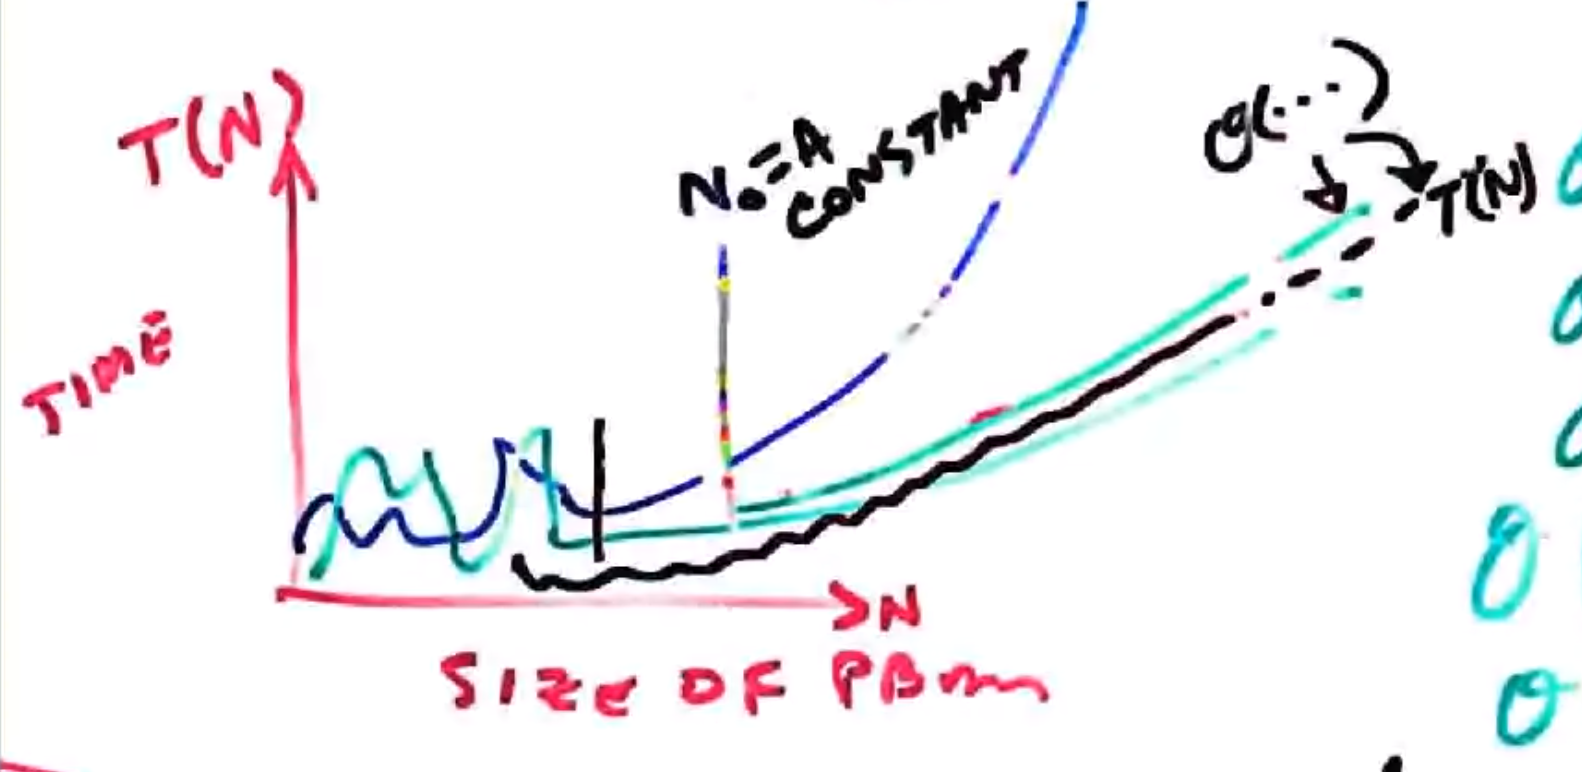
\includegraphics[width=13.8cm]{big_o.png}}
%       \caption{Big(O) Notation}
%   \end{figure}

%   \begin{lstlisting}[language=Python] 
%        print('hello world') 
%   \end{lstlisting}  

